\subsection{Verwandte Arbeiten}
\begin{frame}
  \frametitle{\currentsectionname}

  \begin{itemize}
    \item \textit{Scratch}, \textit{Snap!} und \textit{DataSnap}: aufeinander aufbauende visuelle Programmierumgebungen.
      \begin{itemize}
        \item Blockformen bestimmen Kombinationsmöglichkeiten.
        \item \textit{Scratch} und \textit{Snap!}: Erlernen von Programmierkonzepten.
        \item \textit{DataSnap} richtet sich an Fachexpert:innen, die Daten verarbeiten wollen.
      \end{itemize}
    % \item \textit{DBSnap}: Anwendung zum Erstellen von Datenbankabfragen, welche die relationale Algebra mit Bausteinen darstellt.
    % \item \textit{SQheLper}: Generierung von SQL-Abfragen durch das Zusammensetzen von Blöcken.
    \item \textit{Home Assistant}: kostenlose und quelloffene Plattform zur Steuerung von Smart Homes.
  \end{itemize}

  \Note{
  \item Scratch, Snap und Datasnap nutzen alle Blöcke, die mit Formen zusammensetzbar sind
  \item Scratch primär an 8- 16-jährige gerichtet, Snap! soll sogar in der höheren Bildung genutzt werden können
  \item Home Assistant: Definition von Automatisierungen und Skripten über blockbasiertes Interface
  \item Inspiration für Design
  }

\end{frame}

% \begin{frame}
%   \frametitle{Scratch}
%
%   \begin{figure}
%     \begin{center}
%       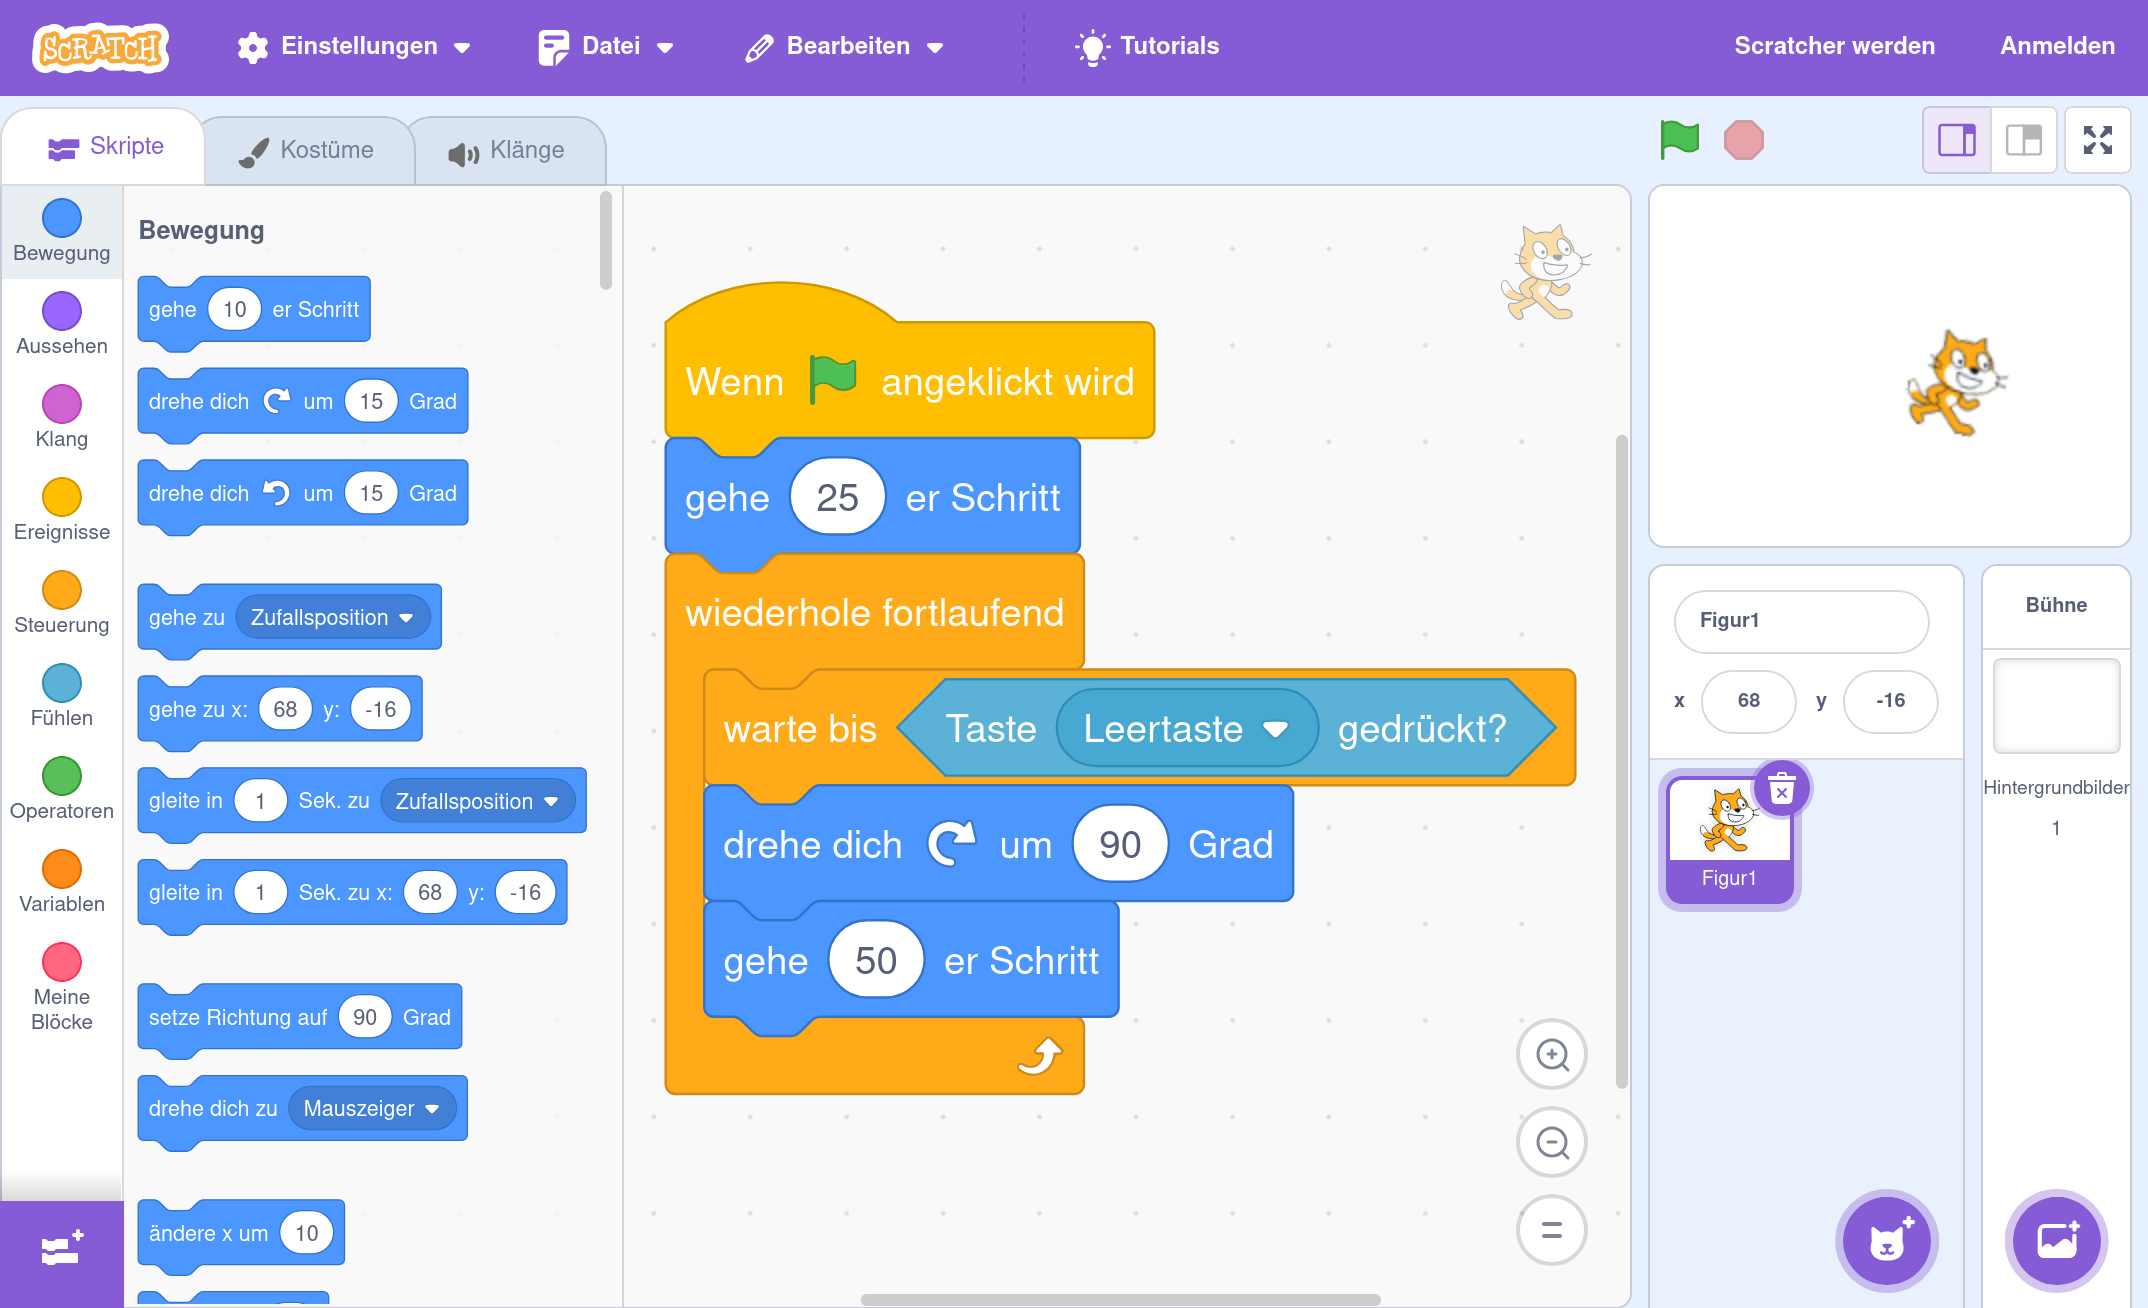
\includegraphics[height=0.7\textheight]{assets/scratch.png}
%     \end{center}
%     \caption{Die Programmierumgebung \textit{Scratch} mit einem Beispielprogramm.}
%   \end{figure}
%
%   \Note{
%   \item Visuelle Programmierungumgebung zum Erlernen von Programmierkonzepten
%   \item primär an 8- bis 16-jährige Kinder gerichtet
%   \item Auswählbare Blöcke links
%   \item Programm in der Mitte zusammensetzen
%   \item Output auf der rechten Seite
%   }
%
% \end{frame}

\begin{frame}
  \frametitle{Snap!}

  \begin{minipage}{.6\textwidth}
    \begin{itemize}
      \item Neuimplementierung von \textit{Scratch} mit neuen Funktionen.
      \item Unterstützt Rekursion und komplexere Datenstrukturen.
      \item Soll auch zur Lehre in der höheren Bildung geeignet sein.
    \end{itemize}
  \end{minipage}%
  \begin{minipage}{.4\textwidth}
    \begin{figure}
      \begin{center}
        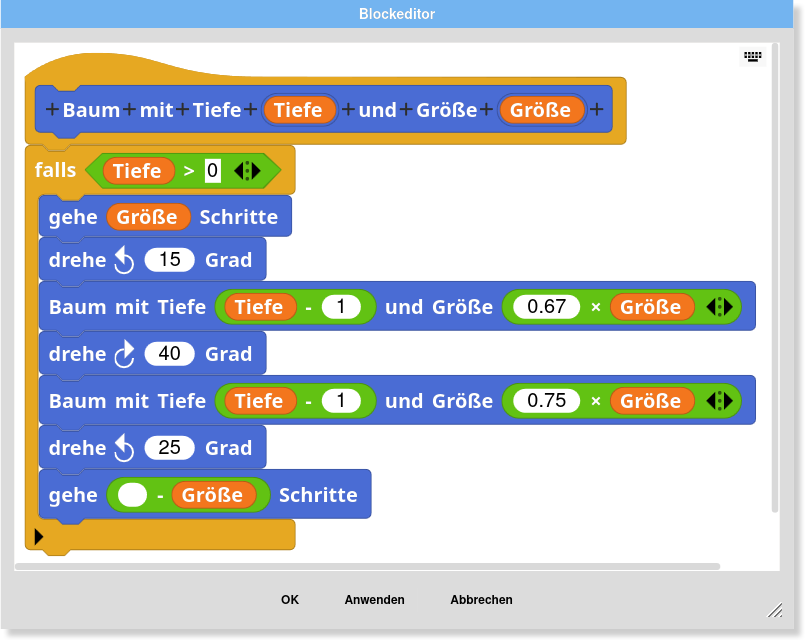
\includegraphics[width=0.95\textwidth]{assets/snap-edit.png}
      \end{center}
      \caption{Definition einer Funktion in \textit{Snap!}.}
    \end{figure}
  \end{minipage}

  \Note{
  \item Scratch primär an 8- 16-jährige gerichtet
  \item rekursive Funktion, die Baum zeichnet
  }

\end{frame}

\begin{frame}
  \frametitle{DataSnap}

  \begin{minipage}{.6\textwidth}
    \begin{itemize}
      \item Weiterentwicklung von \textit{Snap!}, die an Fachexpert:innen gerichtet ist.
      \item Einfaches Importieren von Daten.
      \item Nutzung von externen Rechnern zur Beschleunigung der Auswertung.
      \item Benutzung von \textit{Snap!}-Blöcken zur Definition der Datenverarbeitung.
    \end{itemize}
  \end{minipage}%
  \begin{minipage}{.4\textwidth}
    \begin{figure}
      \begin{center}
        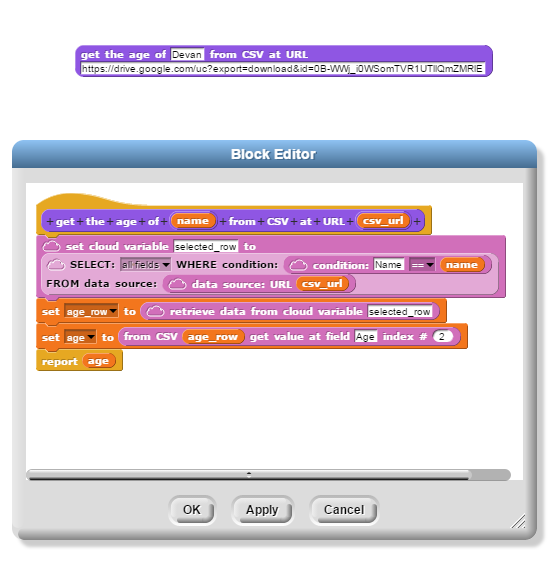
\includegraphics[width=0.95\textwidth]{assets/datasnap-block-definition.png}
      \end{center}
      \caption{Definition eines Blocks in \textit{DataSnap}. \parencite[26]{hellmannDataSnapEnabling2015}}
    \end{figure}
  \end{minipage}

  \Note{
    \item Masterarbeit
    \item Importieren über diesen dunkelpinken Block "data source"
    \item Abspeichern in sog. cloud variablen - auf externem Rechner, also Server
    \item auf dem Server können dann auch Berechnungen ausgeführt werden, weniger abhängig vom Client
    \item Hier rechts wird die Funktionalität als Block definiert, um später in anderen Abfragen schnell wiederverwendet zu werden
  }

\end{frame}

\begin{frame}
  \frametitle{DataSnap (2)}

  \begin{itemize}
    \item Visualisierung der Ergebnisse.
  \end{itemize}
  \begin{figure}
    \begin{center}
      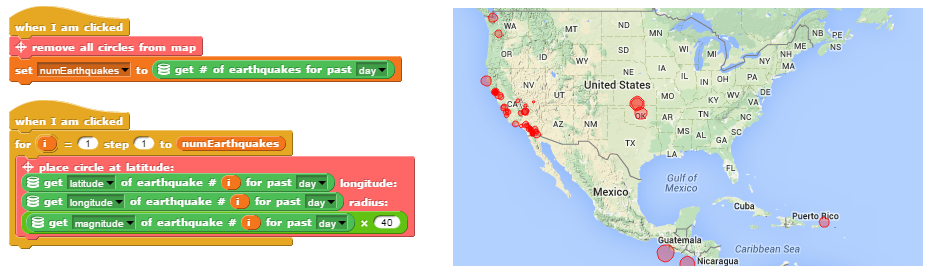
\includegraphics[width=0.95\textwidth]{assets/datasnap-visualization.png}
    \end{center}
    \caption{Visualisierung von Erdbeben mit \textit{DataSnap}. \parencite[28]{hellmannDataSnapEnabling2015}}
  \end{figure}

  \Note{
    \item mithilfe von standard Snap! und neu eingeführten Blöcken Visualisierung möglich
    \item Hier z.B. Erdbeben in Nordamerika mit Darstellung der Magnitude in Form des Radius der Kreise
  }

\end{frame}
